\documentclass[11pt,letterpaper]{article}

\usepackage{graphicx}
\usepackage[margin=1in]{geometry}
\usepackage{amsmath}
\usepackage[T1]{fontenc}
\usepackage[utf8]{inputenc}
\usepackage{authblk}
\usepackage{fancyhdr}
\usepackage{lastpage}
\usepackage[parfill]{parskip}
\usepackage{subcaption}

\pagestyle{fancyplain}
\fancyhf{}
\fancyfoot[R]{\footnotesize Page \thepage\ of \pageref{LastPage}}

\renewcommand{\headrulewidth}{0.0pt} % No header rule
\renewcommand{\footrulewidth}{0.4pt} % Thin footer rule

\begin{document}

\title{Visual Discovery of Communication Patterns in Email Networks}

\author[ ]{Benjamin Bengfort}
\author[ ]{Konstantinos Xirogiannopoulos}
\affil[ ]{Department of Computer Science}
\affil[ ]{University of Maryland}
\affil[ ]{\textit{\{bengfort,kostasx\}@cs.umd.edu}}

\date{April 6, 2015}

\maketitle

\section*{Introduction}

Use Gephi \cite{gephi_gephi-open_2010} to visualize the network from a GraphML \cite{brandes_graph_2010} file. Gephi is used for visual exploration and mapping of networks \cite{bastian_gephi:_2009} and can do statistical analysis of small to medium networks \cite{mcsweeney_gephi_2009}.

Force Atlas 2 Continuous Layout \cite{jacomy_forceatlas2_2014}

Louvian Community Detection \cite{de_meo_generalized_2011}

Edge Bundling \cite{pupyrev_edge_2012}

Dynamic network connections within Twitter conversations are explored in \cite{bruns_how_2012}.

Email is the most prominent form of communication of our time. We use email for both proffessional, as well as casual communication throughout daily life. Such large amounts of time spent on writing, reading and responding to email, yet email comes and goes, without there really being a way for users to have a slightly higher level overview of what groups of people they are communicating with or how often they are communicating with them. Therefore, for this assignment we decided to provide visualizations of our email networks. We believe that visualizing email networks are a great choice for this project as they will provide a broader overview of what our communication clusters look like, as well as allow insight about who the key-players are in our networks, and who are the ones  who have brought us closer to other people.

\subsection*{Using Email as a Dataset}

\begin{figure}[h]
	\centering
	\begin{subfigure}{0.49\textwidth}
		\centering
		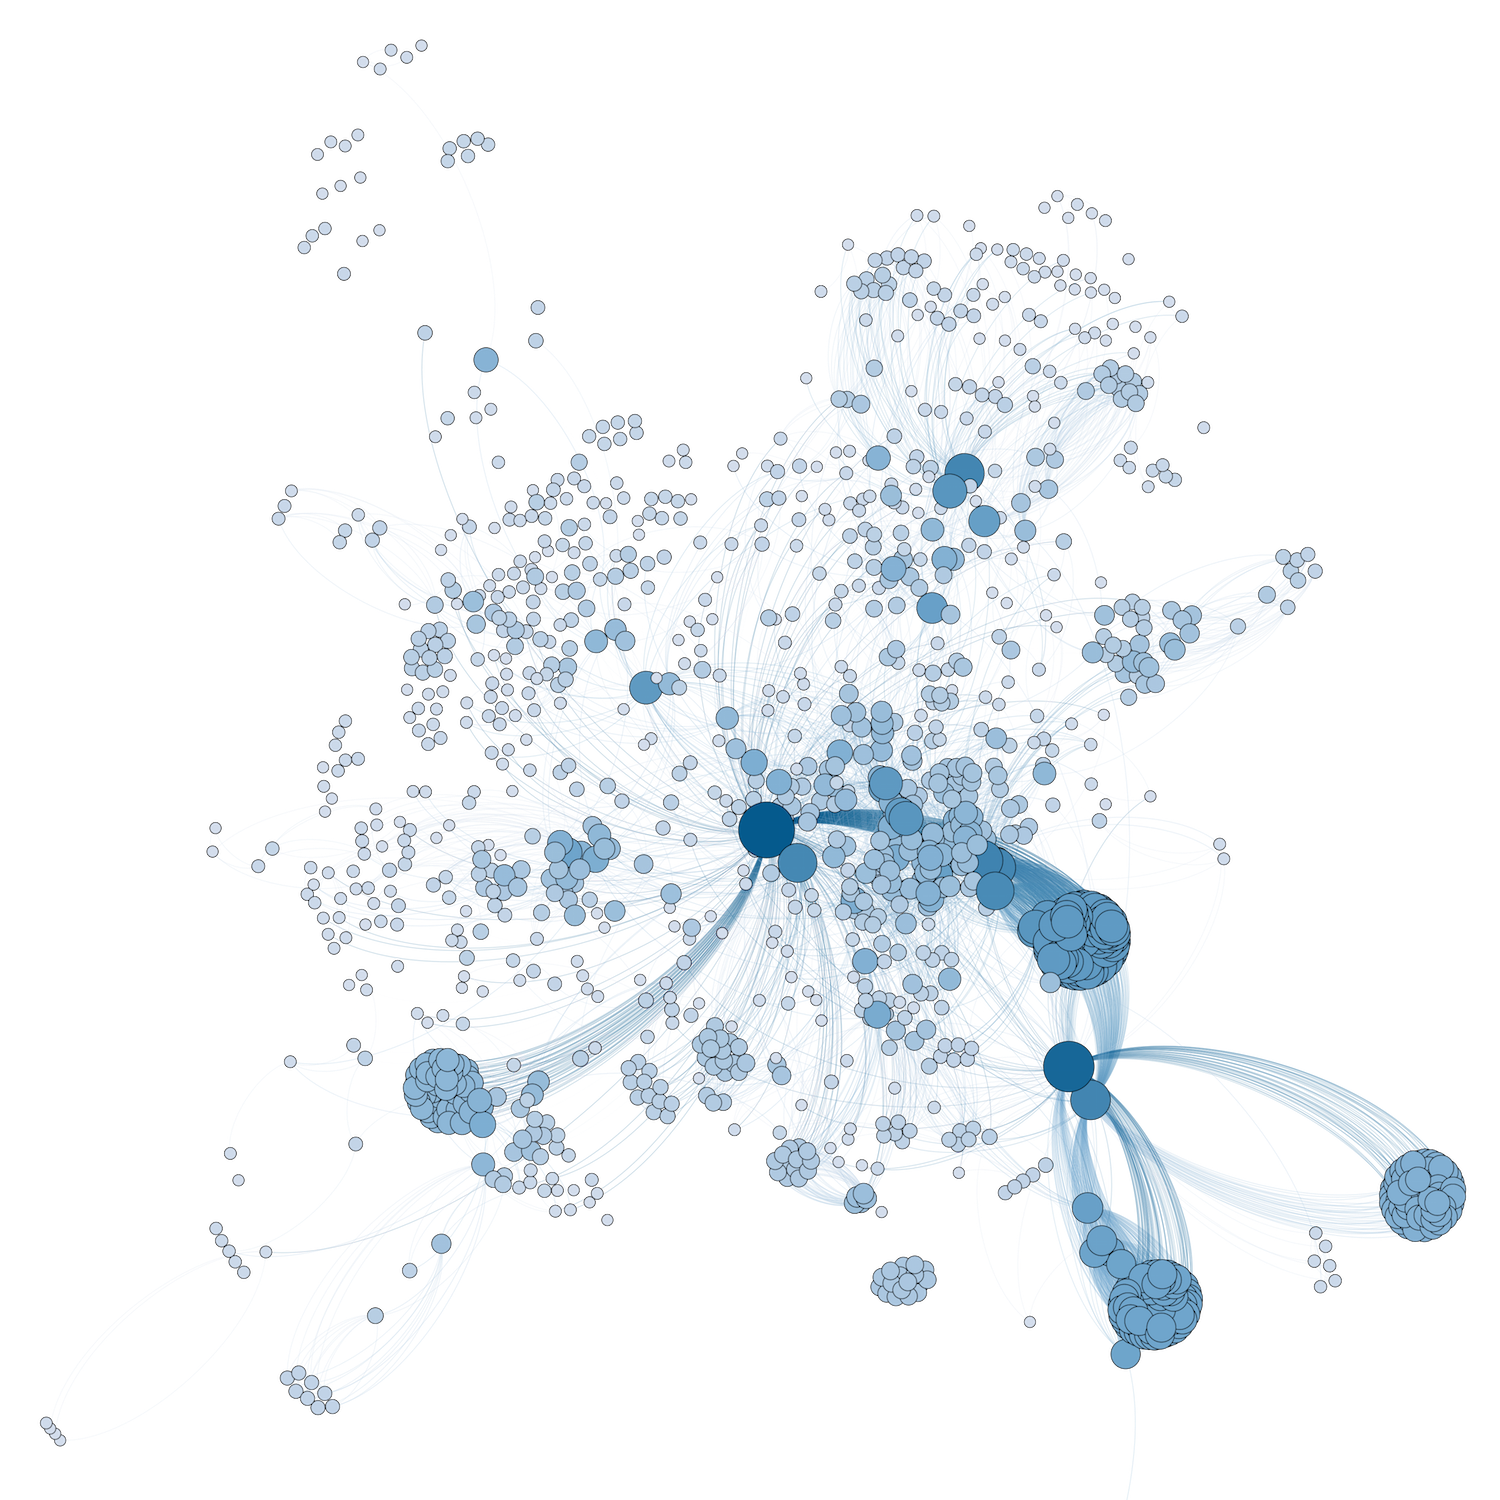
\includegraphics[width=\textwidth]{figures/benjamin_descriptive.png}
		\caption{\textsf{Benjamin Bengfort (Large)}}
        \label{fig:benjamin_descriptive}
	\end{subfigure} \hfill
	\begin{subfigure}{0.49\textwidth}
		\centering
		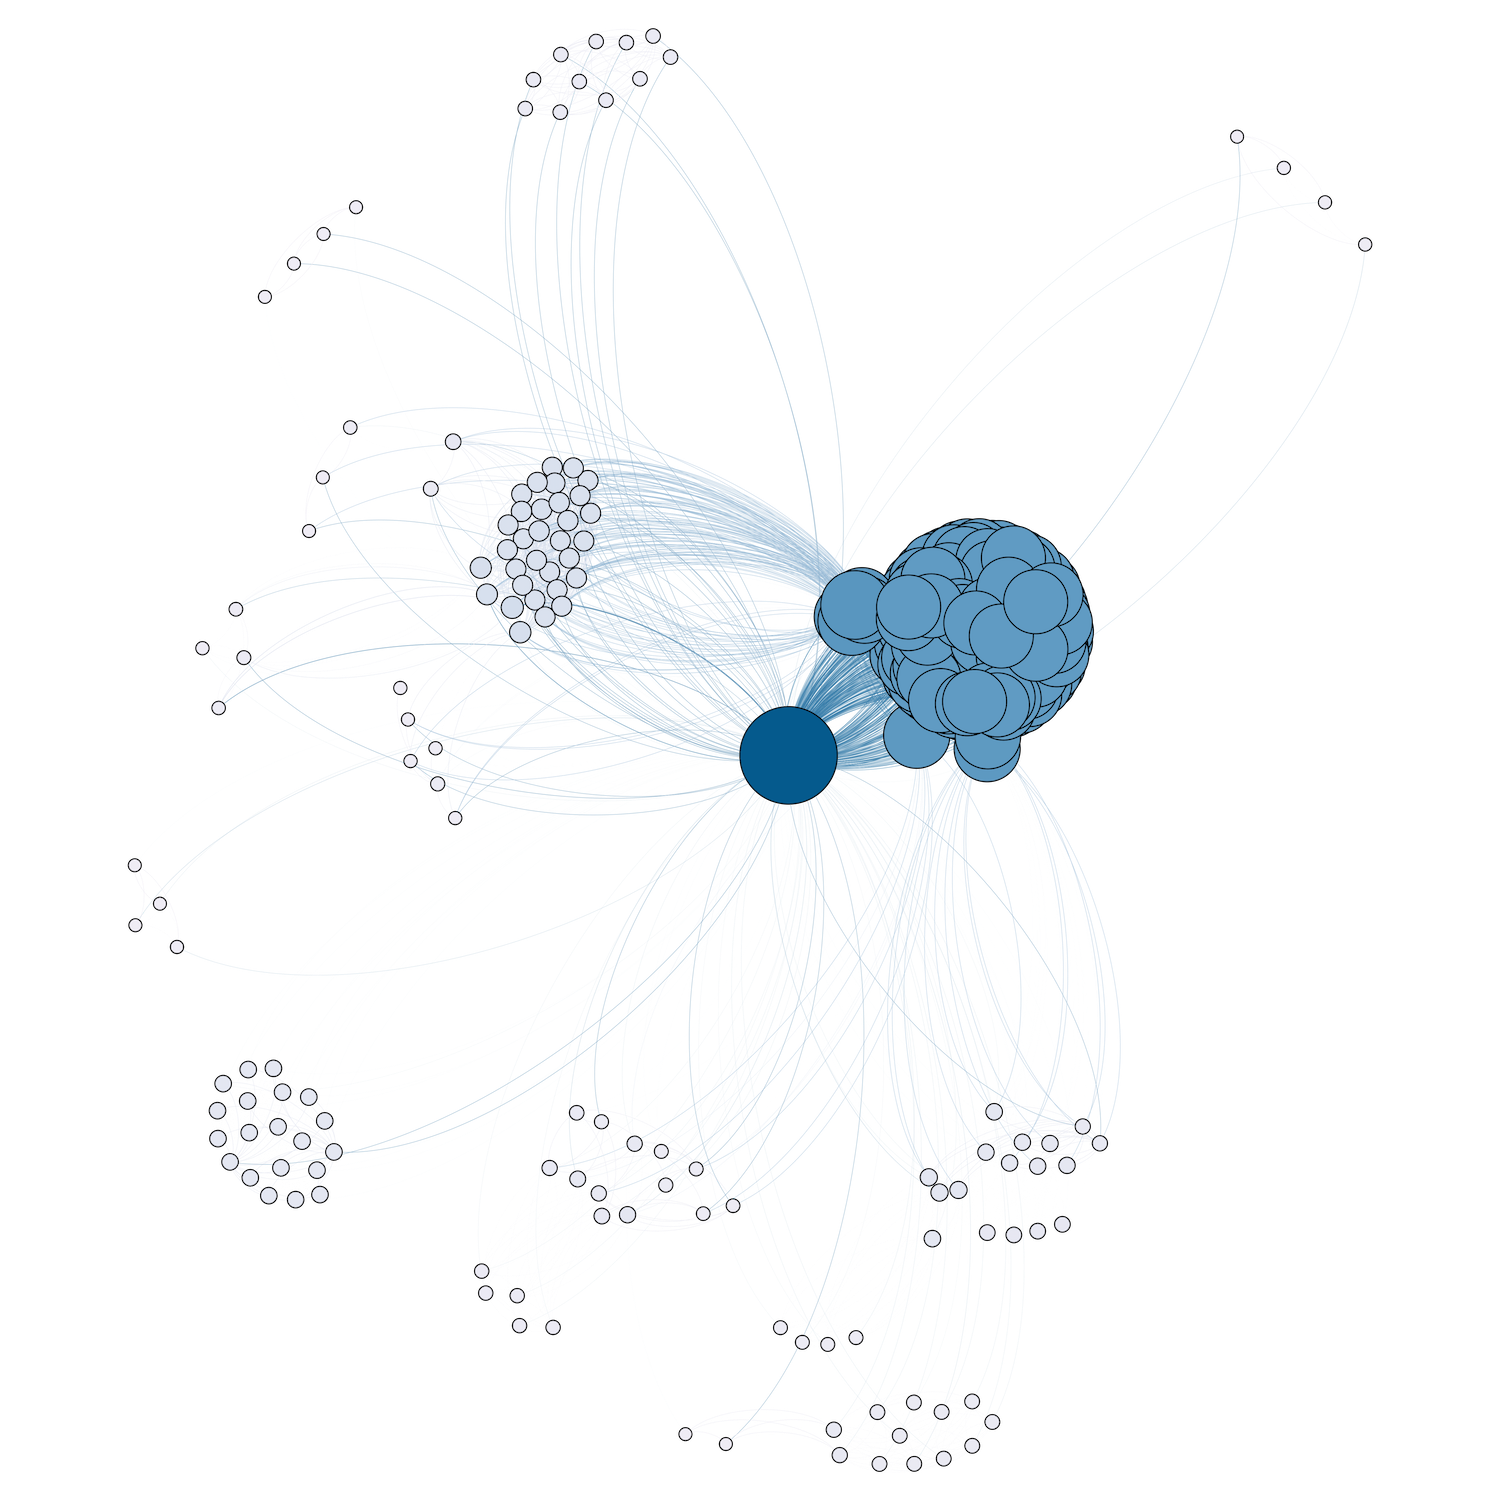
\includegraphics[width=\textwidth]{figures/kostas_descriptive.png}
		\caption{\textsf{Konstantinos Xirogiannopoulos (small)}}
        \label{fig:kostas_descriptive}
	\end{subfigure}
    \caption{\textsf{Email networks, no matter the size are complex.}}
    \label{fig:descriptive}
\end{figure}

Describe the nodes, edges, density and other network characteristics of the GraphML file.

In email netowrks, the nodes represend the unique email addresses of the individuals who participate in the network. Two individuals in the network share an edge if they have somehow participated in a conversation. That includes direct emails that the center node has perticipated in, wether they play the role of the receiver or the sender. The thickness of each edge dictates the amount of back and forth communication between the two nodes (the number of email exchanged).

\begin{table}[t!]
    \centering
    \label{tab:network_comparison}
    \begin{tabular}{l | c c}
        \hline
        Metric & Benjamin & Kostas \\
        \hline
        Emails & 52,716 & 9879 \\
        Nodes & 3,408 & 1,005 \\
        Edges & 37,158 & 56,370 \\
        Avg. Degree & 21.8063 & 112.1791 \\
        \hline
    \end{tabular}
    \caption{Description of Email Datasets}
\end{table}

For the sake of comparison and diversity in our examples, we have extracted both of our email networks, and ran the same statistics on them. This will allow for more concrete and reliable insight on how network visualization can yield very important insights on vast and complex interconnected data.

\subsection*{Data Wrangling for Gephi}

Describe using Python for computation and wrangling, and the tribe script to extract a graph out of an MBox.

\section*{Insights}
%Since we have a seperate section for the headlines, I don't think this section is necessairy. We just talk about the insights in every headline...
In this section we describe the exploration of the email graphs of the authors - both independently and joined using Gephi.

\subsection*{Headline 1}

Explore motif simplification (complexity reduction) using edge Bundling

\begin{figure}[h]
	\centering
	\begin{subfigure}{0.49\textwidth}
		\centering
		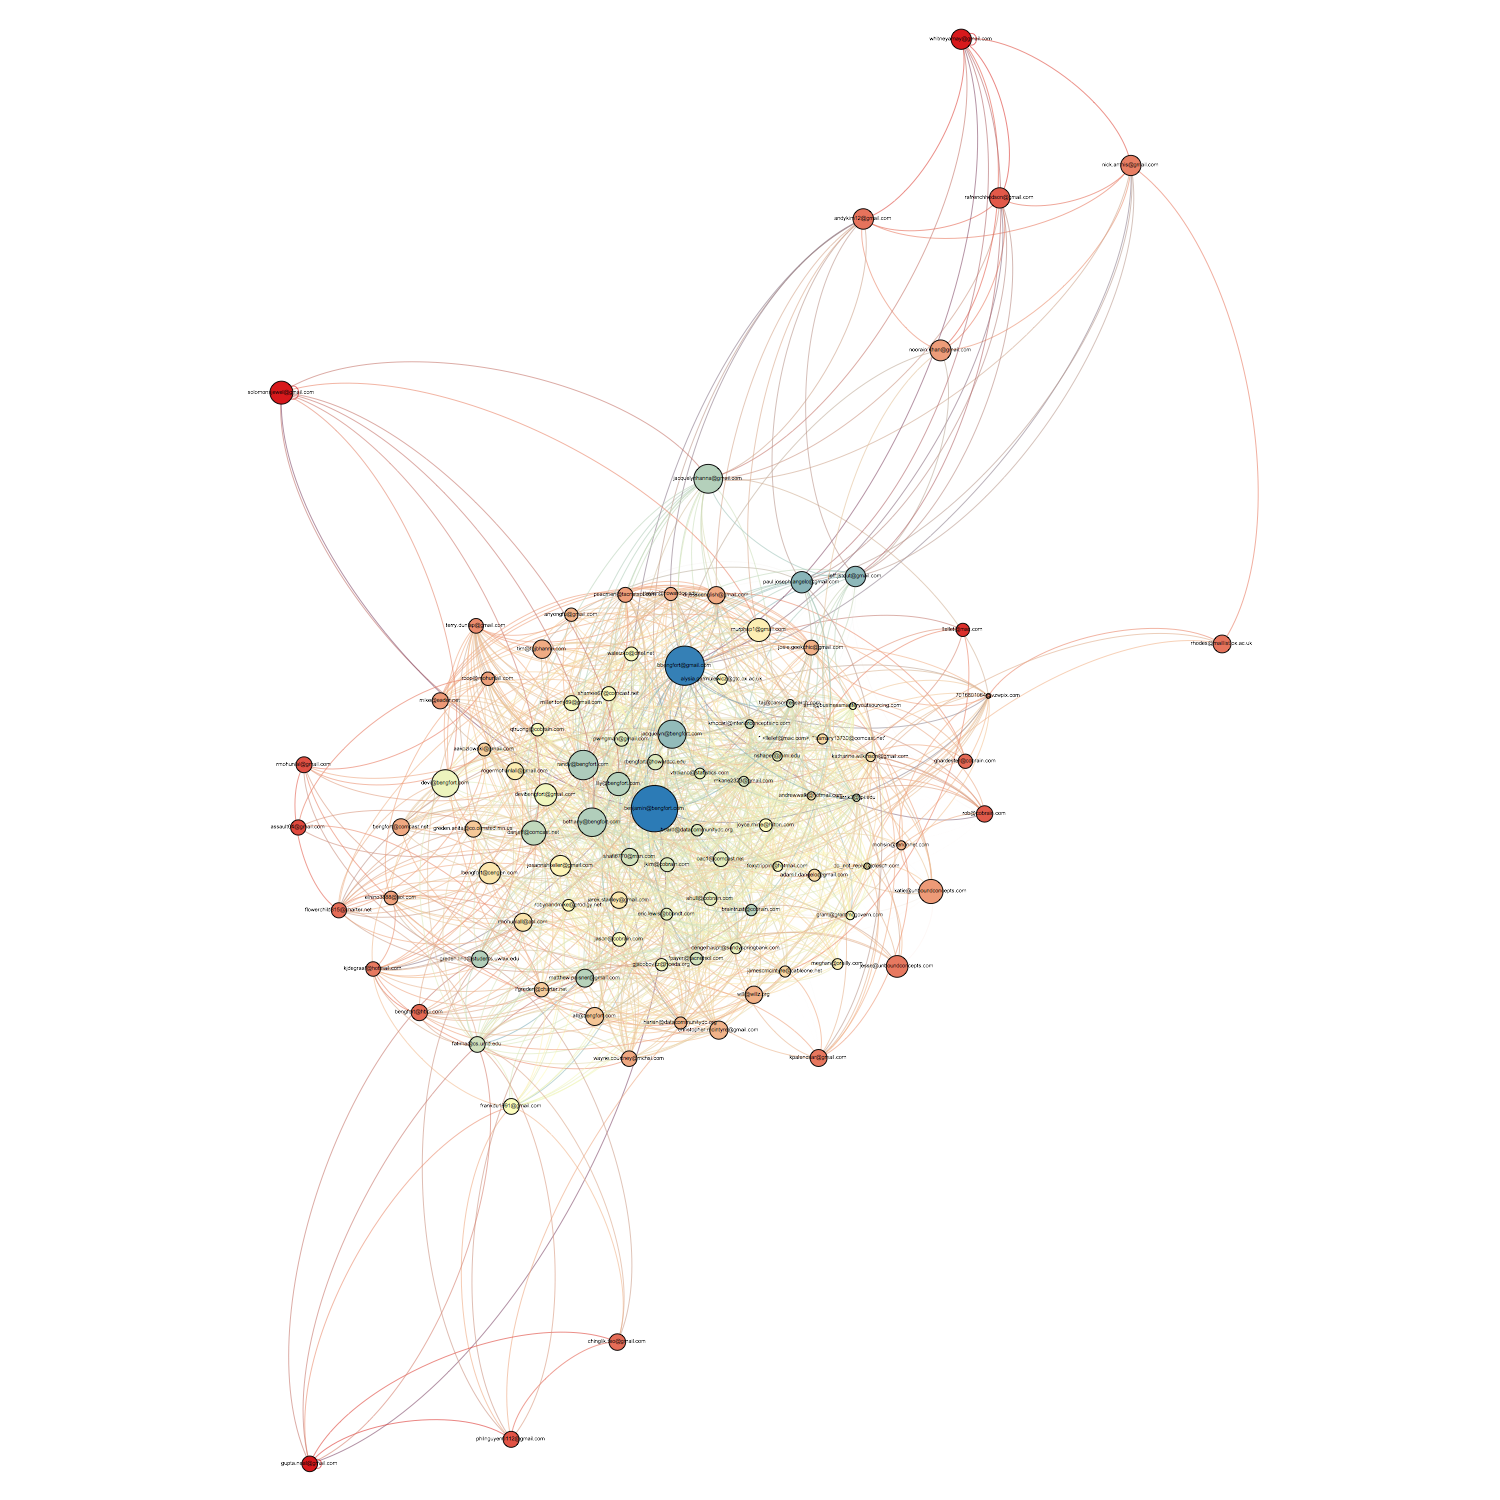
\includegraphics[width=\textwidth]{figures/benjamin_simplification.png}
		\caption{\textsf{Benjamin Bengfort (Large)}}
        \label{fig:benjamin_simplification}
	\end{subfigure} \hfill
	\begin{subfigure}{0.49\textwidth}
		\centering
		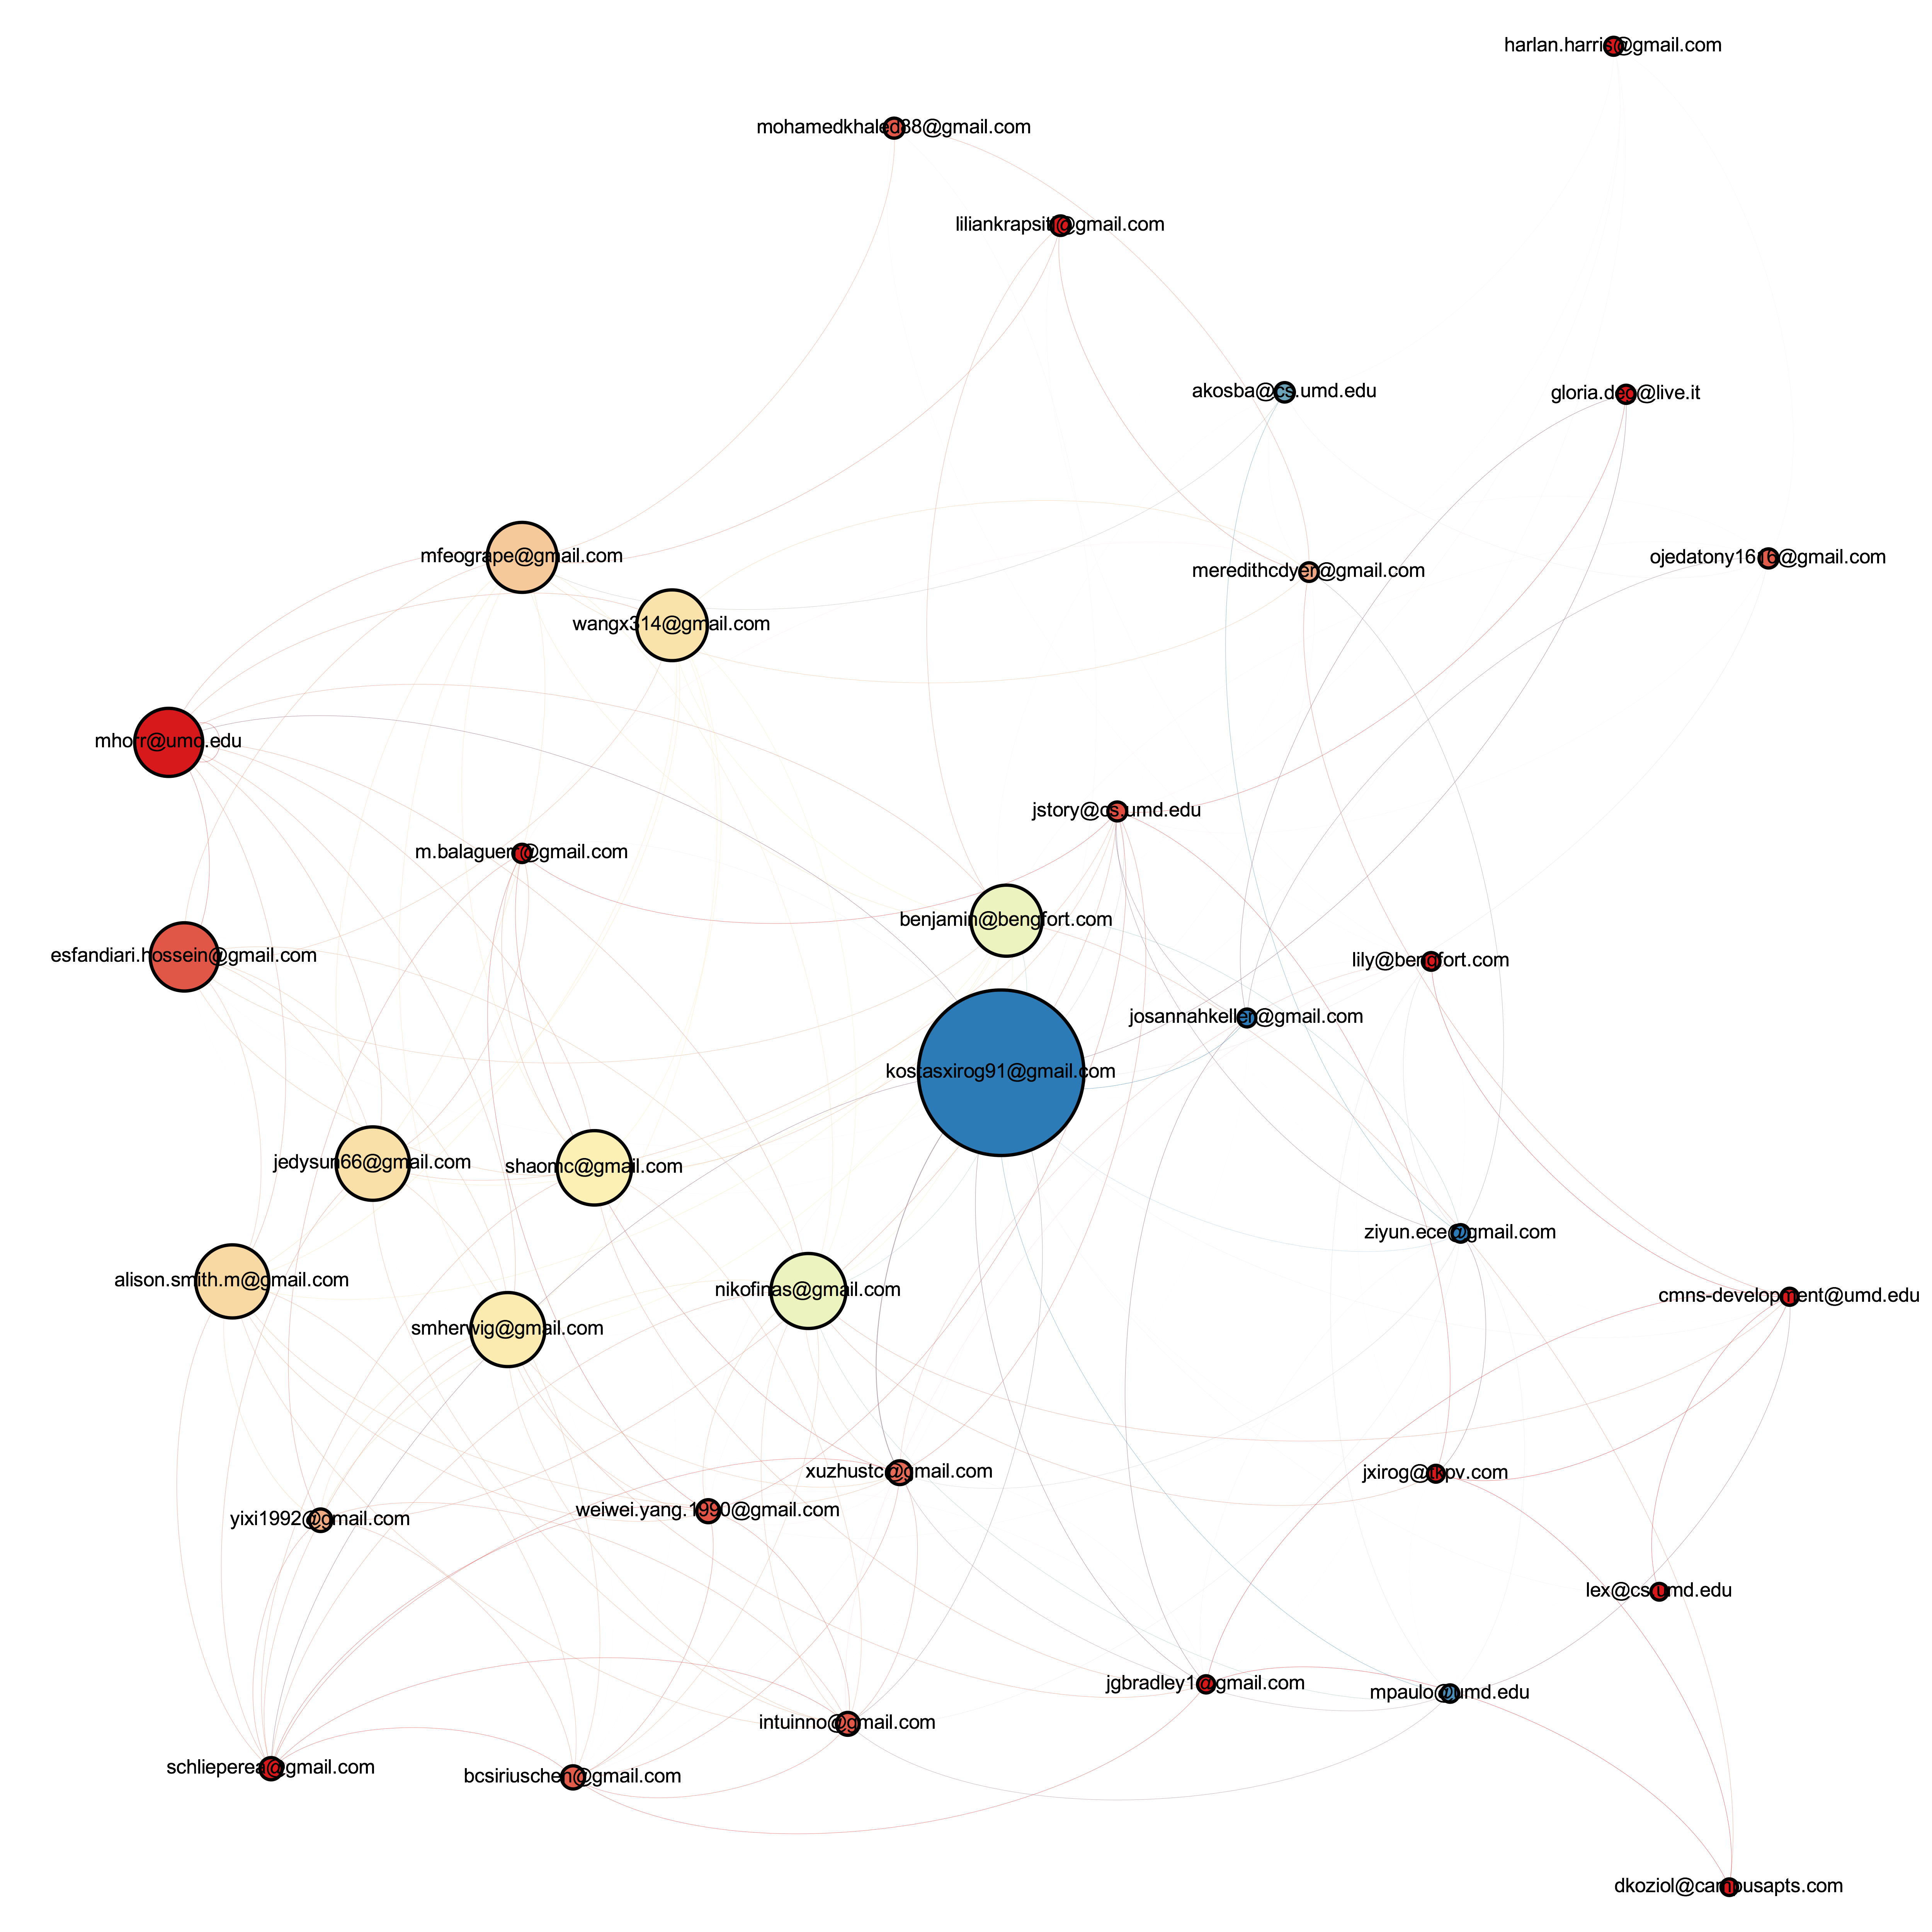
\includegraphics[width=\textwidth]{figures/kostas_simplification.png}
		\caption{\textsf{Konstantinos Xirogiannopoulos (small)}}
        \label{fig:kostas_simplification}
	\end{subfigure}
    \caption{\textsf{Grouping by "Hub" reveals a simpler graph with interesting communication flows.}}
    \label{fig:simplification}
\end{figure}

\subsection*{Headline 2}

Explore centrality measures
% [My idea here, is to remove the center node (ourselves) and explore centrality measures between our interconnected clusters. We could figure out key players using Betweenness centrality. I have also figured this out in gephi in case you don't know how to do it.]

\begin{figure}[h]
	\centering
	\begin{subfigure}{0.49\textwidth}
		\centering
		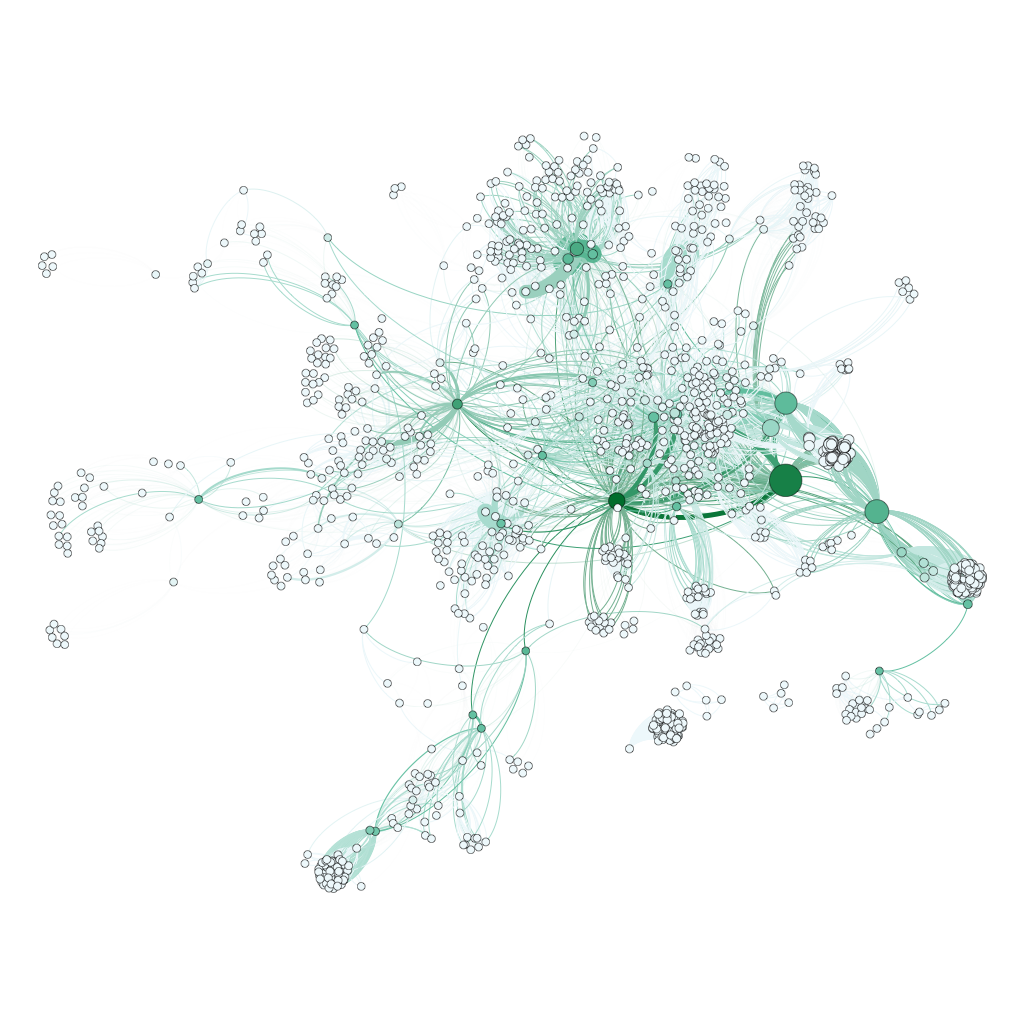
\includegraphics[width=\textwidth]{figures/benjamin_centrality.png}
		\caption{\textsf{Benjamin Bengfort (Large)}}
        \label{fig:benjamin_centrality}
	\end{subfigure} \hfill
	\begin{subfigure}{0.49\textwidth}
		\centering
		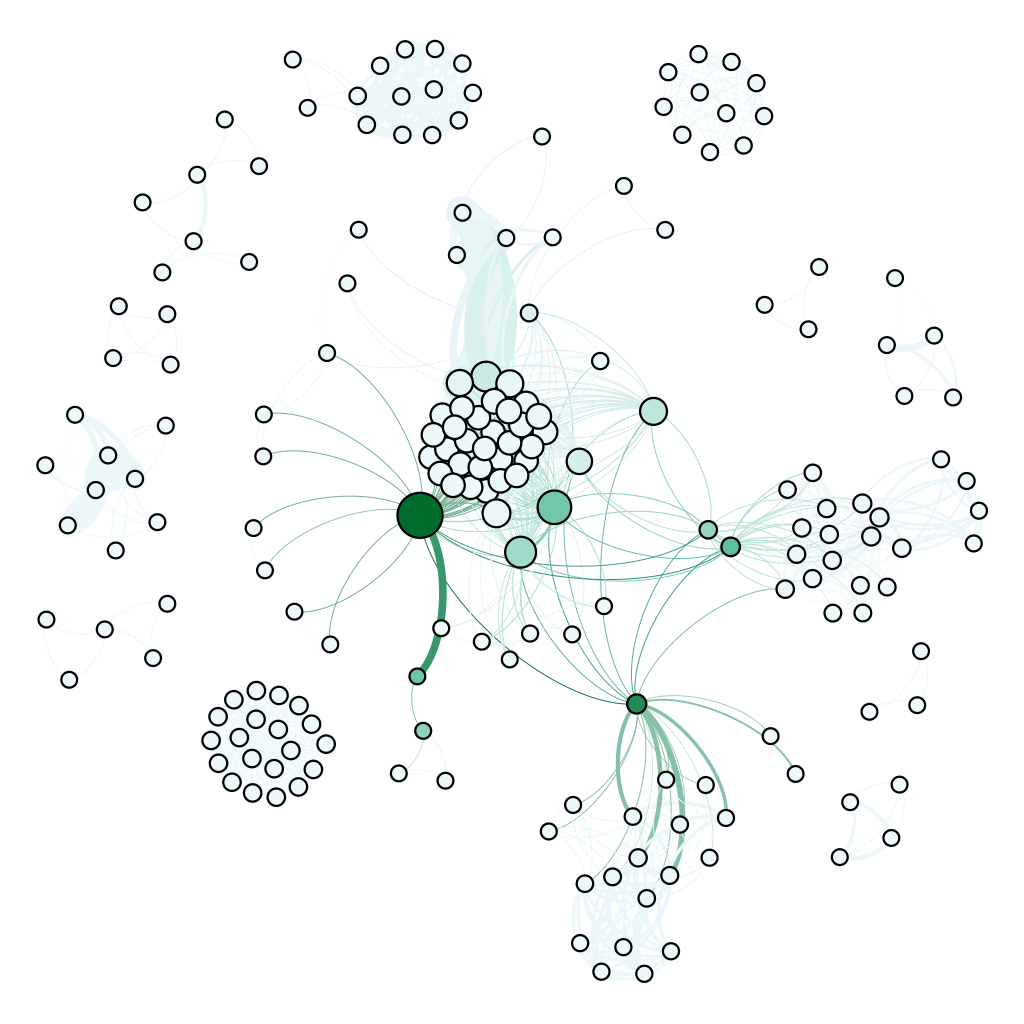
\includegraphics[width=\textwidth]{figures/kostas_centrality.png}
		\caption{\textsf{Konstantinos Xirogiannopoulos (small)}}
        \label{fig:kostas_centrality}
	\end{subfigure}
    \caption{\textsf{Nodes highlighted for their high betweenness centrality}}
    \label{fig:centrality}
\end{figure}

\subsection*{Revealing Clusters and Communities}
% [Here, we will have our two networks, where we show clusters in them, and compare/contrast the two different networks and the clusters that appear within. I have figured out how to do that and I think it looks cool and will show you my network soon]

\begin{figure}[h]
	\centering
	\begin{subfigure}{0.49\textwidth}
		\centering
		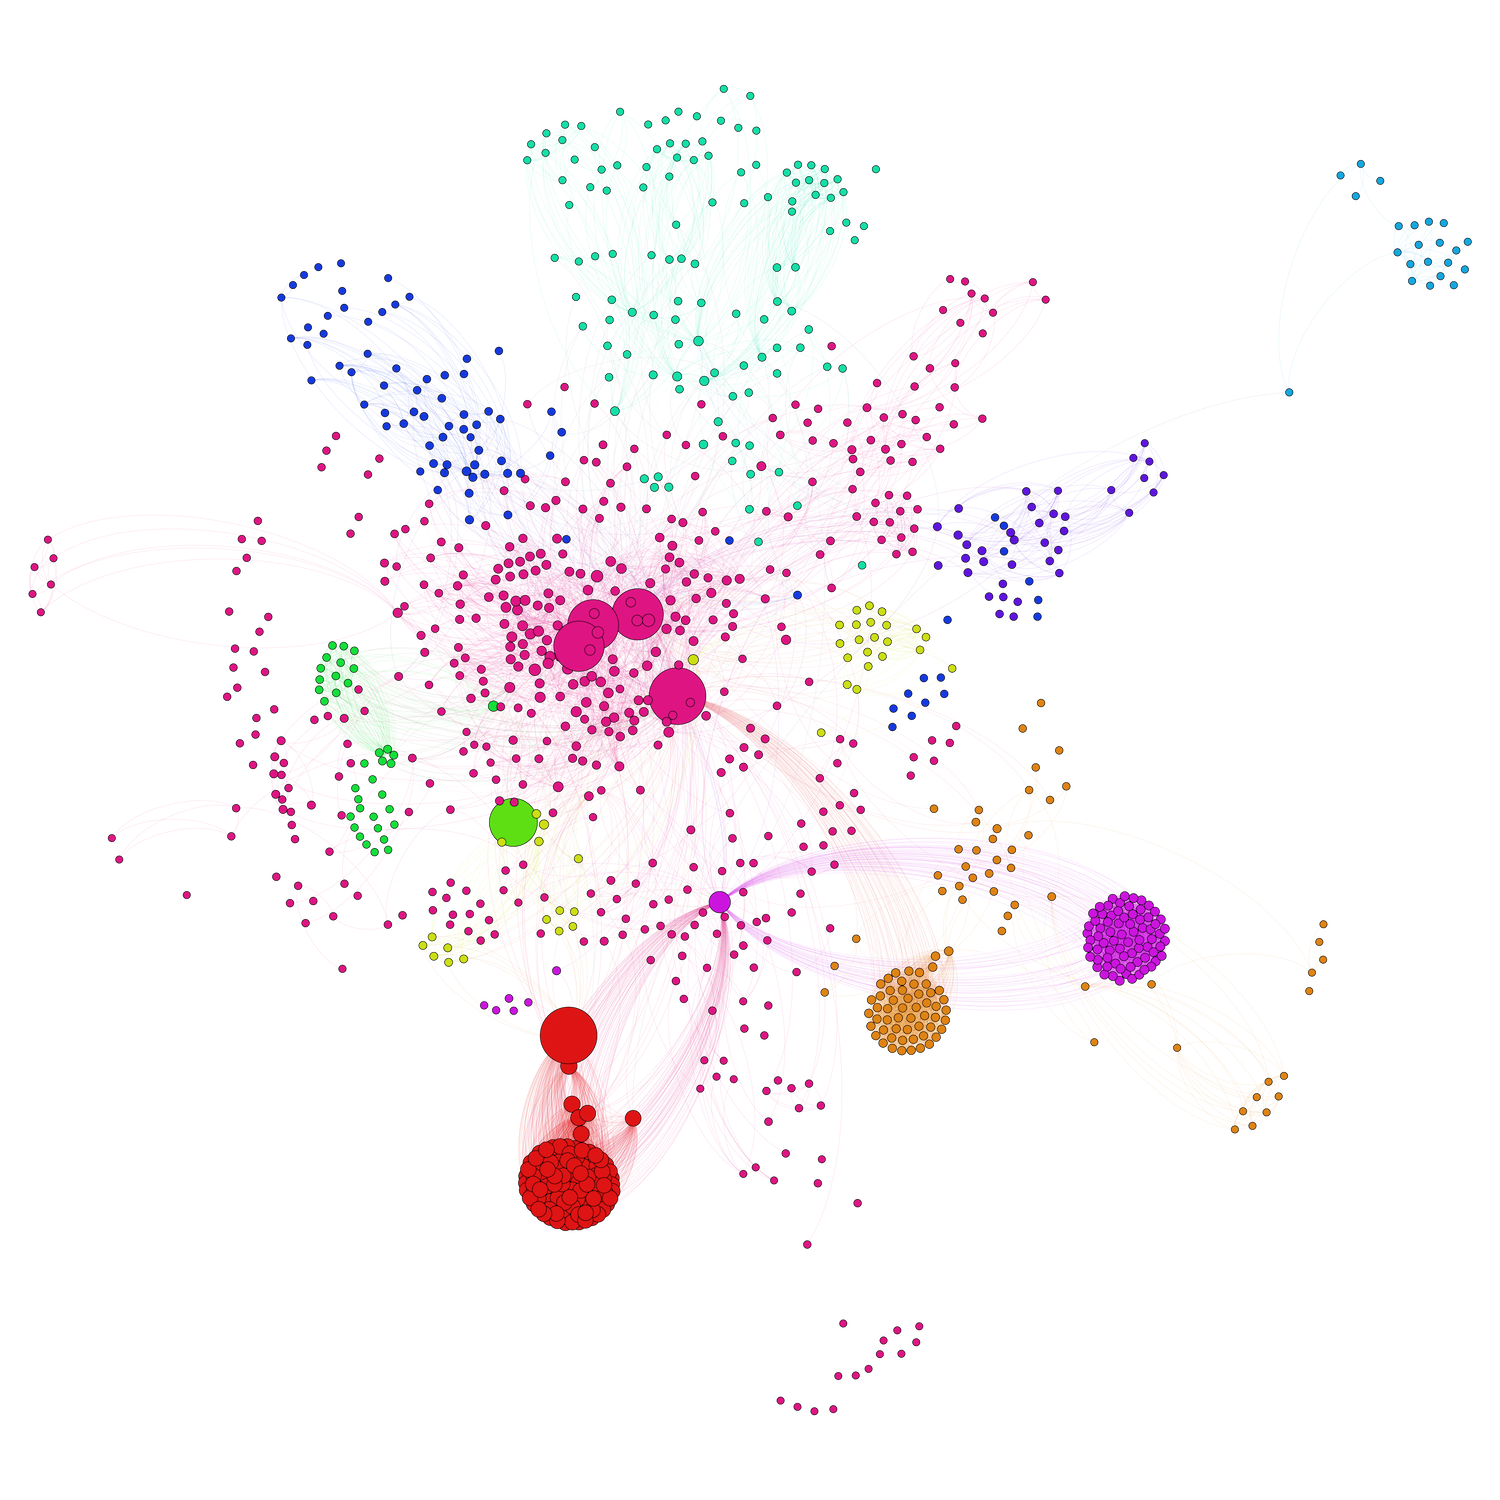
\includegraphics[width=\textwidth]{figures/benjamin_cluster.png}
		\caption{\textsf{Benjamin Bengfort (Large)}}
        \label{fig:benjamin_cluster}
	\end{subfigure} \hfill
	\begin{subfigure}{0.49\textwidth}
		\centering
		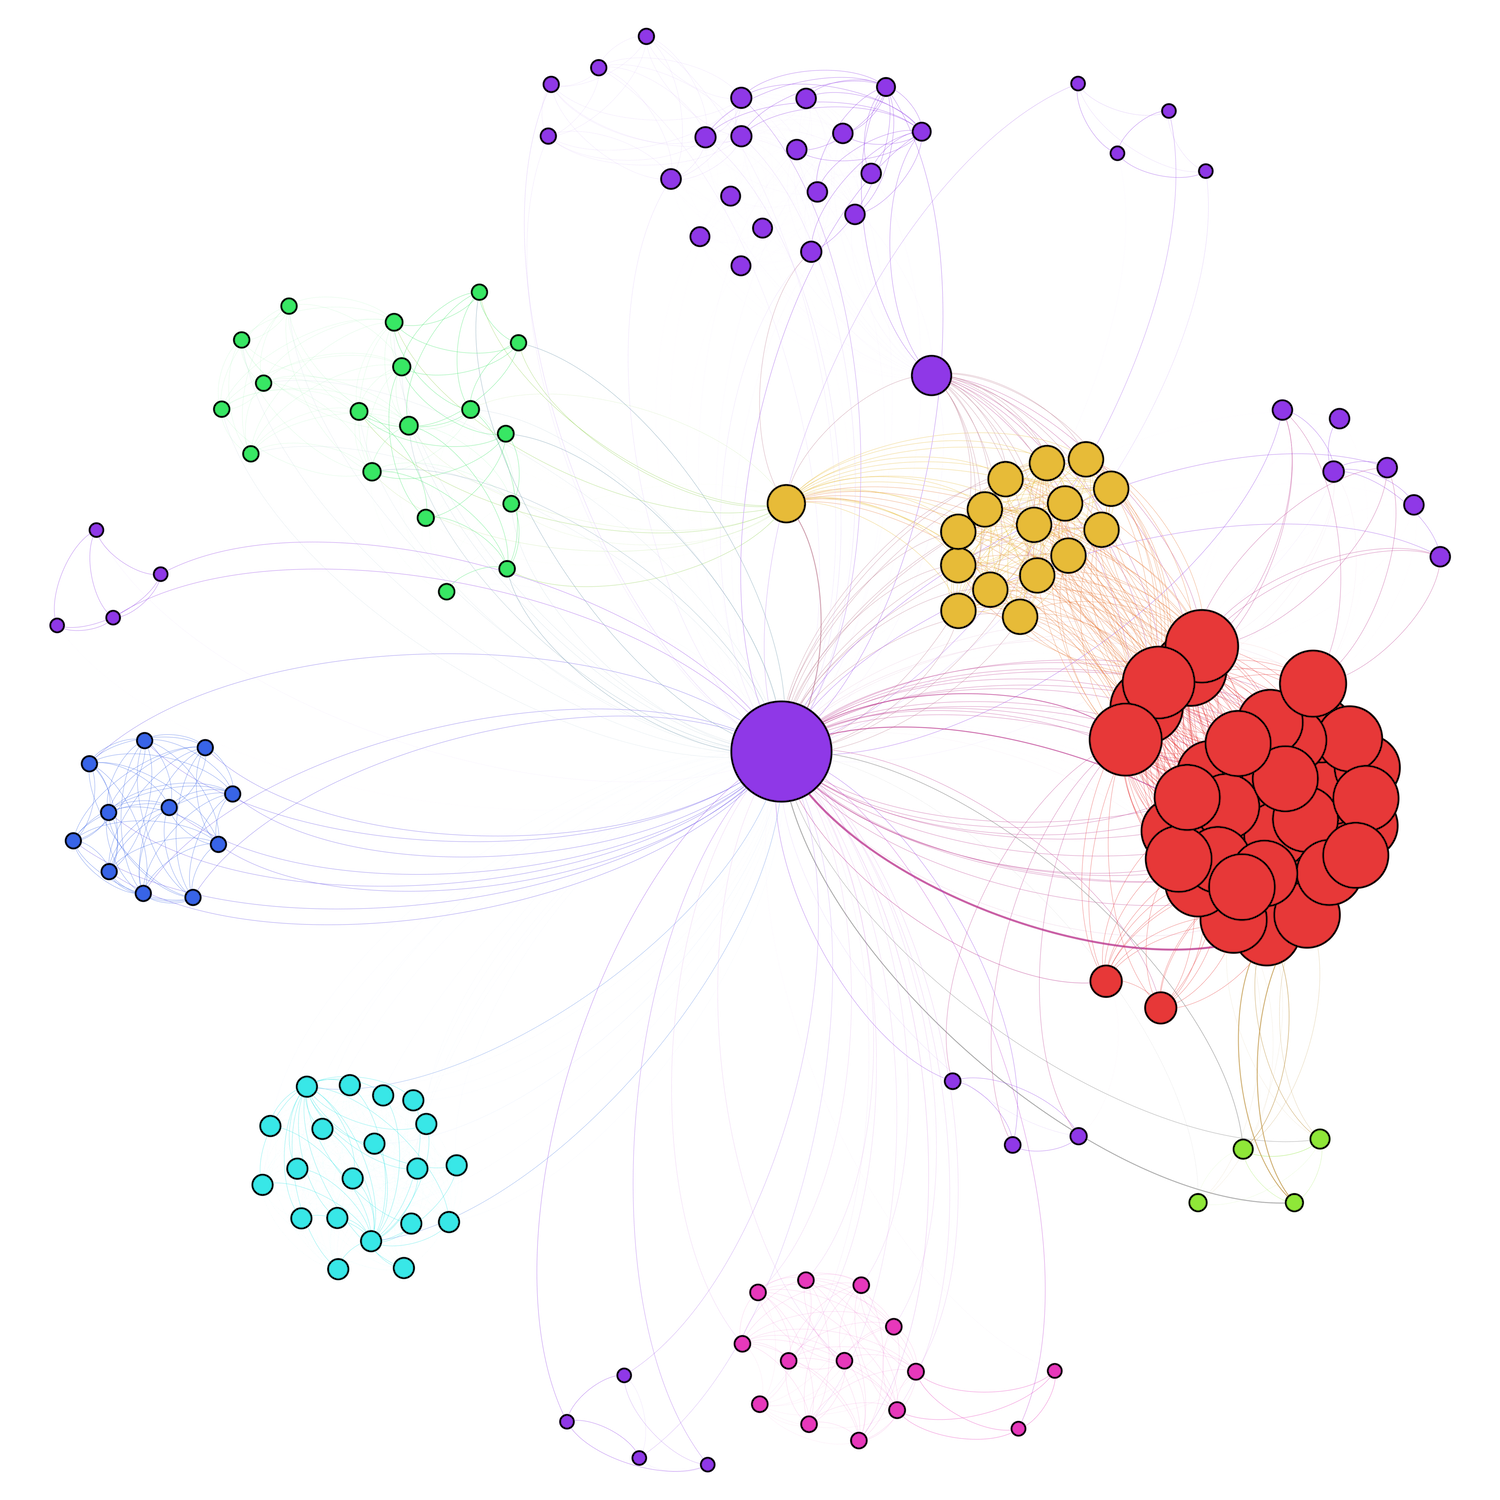
\includegraphics[width=\textwidth]{figures/kostas_cluster.png}
		\caption{\textsf{Konstantinos Xirogiannopoulos (small)}}
        \label{fig:kostas_cluster}
	\end{subfigure}
    \caption{\textsf{Clusters (modularity) colored in email network.}}
    \label{fig:cluster}
\end{figure}

By visualizing our email networks in certain ways, and with the help of some useful features that \textit{Gephi} provides, we were able to extract and reason about about the clusters that form around the center node. To reach this result we used \textit{K-Core filtering} to remove the low degree nodes, as well as \textit{modularity} feature to extract the clusters. As seen in [Figure] there are several clusters that form can form, some of which the center node takes place in, but also some that are disconnected from the center node. Some clusters are very loosely connected, while others share very dense sets of connections. By using the Fruchterman Reingold[] layout algorithm, the clusters appear very clearly and in an organized fashion, around the center node. This layout algorithm allows clusters to emerge and by using \textit{Gephi} we were able to then start digging deeper into what these clusters signify. The emails of our contacts are not shown in the visualization in order to maintain privacy, however \textit{Gephi} allows us to view the email adresses of each node as a label.

\subsection*{Small graph}
In the graph on the right, we can clearly make out the clusters that appear in this individual's network. For example, the red cluster is the university email cluster, and includes email that occured during team projects. This cluster is extremely dense, as emails are being sent back and forth between team members, including everyone in the conversation. There are also a few very thick edges in the graph, between the center node and one more node. This signifies vast amounts of email between these two nodes and only between them.


\section*{Critique}

Gephi is certainly not as complete as NodeXL - but a dedicated system rather than a tie into Microsoft Excel made it more easily accessible on other platforms.

\section*{Conclusion}

What we did, what we learned, what we'd do again.

\bibliographystyle{plain}
\bibliography{paper}

\end{document}
